
\subsection{Simulaciones de Monte-Carlo}

Las simulaciones de Monte-Carlo tienen un principio totalmente distinto
de las simulaciones de dinámica, pero se supone que muestrean el mismo
conjunto de configuraciones si las condiciones termodinámicas son las
mismas. Aquí realizaremos una simulación de Monte-Carlo y verificaremos
que similaridad poseen en relación a las simulaciones de dinámica
molecular. El programa para realizar simulaciones de Monte-Carlo es 
{\tt bin/mc}.

Al contrario de MD, MC no tiene tiempo. Hay una generación de posiciones
aleatorias consecutivas, que son aceptadas o no de acuerdo con el
criterio de Metropolis,\\

{\tt 
\hspace{3cm} Si $V(\vec{x}_j) \leqslant V(\vec{x}_i)$, $P(i\to j) = 1$ 

\hspace{3cm} Si $V(\vec{x}_j) > V(\vec{x}_i)$, $P(i\to j) = e^{-(V_j-V_i)/kT}$
}\\\\
El segundo criterio es, numéricamente, satisfecho comparando el
resultado de $e^{-(V_j-V_i)/kT}$ con el sorteo de un número aleatorio
entre 0 y 1. En nuestros ejemplos, $kT=0.6$.

Este procedimiento genera una secuencia de configuraciones, que en la
práctica tiene correlación porque las nuevas configuraciones son
generalmente generadas por perturbaciones de las configuraciones
anteriores. Las perturbaciones tiene que ser escogidas para minimizar la
correlación, al mismo tiempo que la tasa de aceptación sea razonable.
Tasas de aceptación del orden de 20 a 30\% son consideradas ideales. 

Ejecute el programa {\tt bin/mc}. Dos parámetros van a ser solicitados:
la magnitud de las perturbaciones y el número de pasos. Las
perturbaciones de las posiciones son Gaussianas, y la magnitud de
entrada es el desvío estándar. El número de pasos corresponde al número
de nuevas estructuras, no necesariamente aceptadas, generadas.  

Para un número de pasos de 50.000, pruebe diferentes perturbaciones,
hasta que al fin una tasa de aceptación de al rededor de 30\% sea
obtenida. (Algo próximo a $0.08$~\AA). 

Una vez elegida la perturbación, ejecute el programa con número de pasos
de 200.000, lo que implica que aproximadamente 60.000 pasos van a ser
aceptados (para una tasa de 30\%). 

Observe la evolución de la energía potencial. Observe la trayectoria. 
(con los mismos comandos de antes). Deje el gráfico abierto, para
comparación posterior. 

\subsubsection{Comparación con MD}

Ejecute, nuevamente, el programa {\tt bin/md-langevin} con los
parámetros $\lambda=0.01$ y $\Delta t=0.05$. Observe el gráfico
de energías. Compare la energía {\it potencial} de este gráfico con la
energía potencial de la simulación de Monte-Carlo.

\subsubsection{Cálculo de la estructura}

Vamos a comparar la estructura media obtenida usando MD con la
estructura media obtenida con MC. Para eso vamos a usar la función
$g(r)$, que se llama ``función de distribución radial''. 
Esta función mide la probabilidad de encontrar una partícula a
una distancia $r$ de otra partícula en el sistema real, en relación a
esa misma probabilidad si no hubiese ninguna interacción entre las
partículas. 

En nuestro caso bi-dimensional, el número de partículas por unidad de
volumen es $\rho=n/A$, donde $n=100$ es el número de partículas y $A=100^2$
es el área total del sistema simulado. El número de partículas esperado
en un intervalo de distancias entre $r$ y $r+\Delta r$ de cada partícula
es, por lo tanto $n(r)=\rho A(r)$, donde $A(r)$ es el área de una cáscara
circular de radio menor $r$ y radio mayor $r+\Delta r$:
\begin{center}
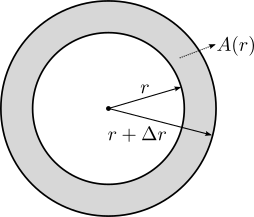
\includegraphics[width=6cm]{./area.pdf}
\end{center}
Vemos que $A(r)=\pi (r+\Delta r)^2 - \pi r^2 \approx 2\pi r\Delta r$.
De este modo, el número de partículas esperado, en media, seria de 
$n(r)=2\pi r\Delta r\rho$, si no hubiese interacciones. 

Las interacciones hacen con que el número de partículas en cada
distancia sea diferente de una distribución homogénea. Si hay
interacciones favorables, por ejemplo, la probabilidad de encontrar dos
partículas próximas es mayor. Esta distribución de partículas es uno de
los parámetros estructurales más importantes.

El programa {\tt bin/gr} calcula, a partir de la trayectoria, la función
$g(r)=n'(r)/n(r)$, done $n(r)$ esta definido anteriormente, y $n'(r)$ es
el número medio de partículas efectivamente observado entre $r$ y $r+\Delta r$
en la simulación. 

Haga una simulación de dinámica molecular con el termostato de Langevin,
ahora por más tiempo, 
usando el comando 
\command{./bin/md-langevin 15000}
Use los parámetros
$\lambda=0.01$ y $\Delta t=0.05$. Observe la trayectoria resultante y
calcule al función $g(r)$ simplemente ejecutando el programa {\tt
bin/gr}. En seguida, visualice el $g(r)$ con
\command{xmgrace gr.dat} 
Mantenga este gráfico abierto, para comparación futura. Entienda que
significa, en función de la visualización de la simulación. 

En seguida, haga una simulación de 200.000 pasos de Monte-Carlo con el programa 
{\tt bin/mc} usando una perturbación de 0.05~\AA. Observe la trayectoria
generada. Ejecute nuevamente el
programa {\tt bin/gr} para obtener la $g(r)$ de esta simulación de
Monte-Carlo. Incorpore los datos al mismo gráfico del $g(r)$ obtenido
por dinámica molecular. Compare. Las simulaciones, con sus naturalezas
totalmente distintas, muestrearon las mismas estructuras?  

\end{document}



















